\chapter{Predictive Modelling}
\hrule
\vspace{40pt}


\section{The Modelling Objective}

Our main aim in this chapter is to predict future mid-price\footnote{Recall in (\ref{mid}) we defined the mid-price, $p_0(t)$ to be the average of the best bid and ask prices at time $t$.}
movement. 
There are multiple possible modelling setups when it comes to mid-price movement prediction.
\cite{KOLM2023} frame this as a regression problem, directly predicting future mid-price values at multiple horizons.
\cite{ZHANG2019} and \cite{LUCCHESE2024} predict the sign of the returns, in a multi-class classification setting.
They argue that due to the highly stochastic nature of financial data, simply calculating labels based on returns from $p_{0}(t)$ and $p_{0}(t+k)$ 
leads to a label set with a lower signal to noise ratio, so smoothed returns are used.

In this paper we use the multi-class classification setup.
Following \cite{ZHANG2019}, we adopt the smoothed labelling method first introduced in \cite{AVRAAM2017}. Define the quantites:
\begin{align}
    m_{-}(t) &:= \frac{1}{k} \sum_{i=0}^{k} p_0(t-i) \\
    m_{+}(t) &:= \frac{1}{k} \sum_{i=1}^{k} p_0(t+i) \\
    \ell(t) &:= \frac{m_{+}(t) - m_{-}(t)}{m_{-}(t)}
    \label{smoothed_returns}
\end{align}
So $m_{-}(t)$ represents the average price for the previous $k$ prices and current price
and $m_{+}(t)$ represents the average price for the next $k$ prices.
Then we calculate the smoothed returns $\ell(t)$ as the return of this smoothed price. 
Then we discretize these returns according to (\ref{desc}) in order to give us three distinct class labels for use in classification.

\begin{equation}
    y(t) = \begin{cases} \label{desc}
        +1  & \text{ if } \ell(t) \in (\epsilon, \infty) \\
        0  & \text{ if } \ell(t) \in [-\epsilon, \epsilon] \\
       -1  & \text{ if } \ell(t) \in  (-\infty, -\epsilon)
   \end{cases}
\end{equation}
So given the information we have up to and including time $t$, our aim is to build a model to predict $y(t)$.

See Figure \ref{fig:example_mid_price_labelling} for a sample of our mid-price data,
colour coded according to class label. We see regions of mid-price downtrend are labelled
with -1 (coloured red), regions of mid-price plateau are labelled with 0 (coloured blue)
and regions of mid-price uptrend are labelled with +1 (coloured green).

\begin{figure}[ht]
    \centering
    \includegraphics[width=1.0\textwidth]{./images/example_labels.pdf}
    \caption{An example BTCUSDT mid-price sample, coloured according to class label.
    Note that the discretization parameter, $\epsilon$ is set $\approx 0$ and the prediction horizon is $k=4$ updates.}
    \label{fig:example_mid_price_labelling}
\end{figure}


Note that in some implementations, the prediction horizon is
given over some time interval, such as predicting the movement for the next 10 seconds.
In this paper, we instead define our prediction horizon in terms of ticks/updates/datapoints.
This choice was made as our WebSocket data arrives at irregular times, and for some short intervals
there is no available data. We expect the results to be very similar when using a time-based horizon.


\section{Model Architecture Background}
In this section we explain the general theory needed for our classification models.

\subsection{Logistic Regression}
Linear regression is one of the oldest and most robust predictive models used in all areas
of science. Its simplicity, explainablity and robustness means it is a common choice for a baseline/benchmark
model.

Logistic regression, first introduced in \cite{COX1958}, is the natural extension of linear regression to the classification setting.
The key idea is to model the \textit{log odds} as linear functions of our data.
Suppose we have $C$ classes, indexed by $1, 2, \cdots, C$, then we assume the following linear model: 
\begin{align*}
    \log \frac{\mathbb{P}(Y=1 | X = x)}{\mathbb{P}(Y=C | X = x)} &= \alpha_1 + \beta_1' x \\
   \log \frac{\mathbb{P}(Y=2 | X = x)}{\mathbb{P}(Y=C | X = x)} &= \alpha_2 + \beta_2' x \\
   \vdots \\
   \log \frac{\mathbb{P}(Y=C-1 | X = x)}{\mathbb{P}(Y=C | X = x)} &= \alpha_{C-1} + \beta_{C-1}' x
\end{align*}
Note that because the probabilities must sum to $1$, we have $C-1$ degrees of freedom.
Also note that the choice of denominator is not important as the model is equivariant
under the choice of denominator class.

With some re-arrangement, we get the posterior probabilities:
\begin{align*}
    \mathbb{P}(Y=c | X = x) &= \frac{\exp(\alpha_c + \beta_c' x)}{1 + \sum_{\ell=1}^{C-1} \exp(\alpha_{\ell} + \beta_{\ell}'x)} \\
    \mathbb{P}(Y=C | X = x) &= \frac{1}{1 + \sum_{\ell=1}^{C-1} \exp(\alpha_{\ell} + \beta_{\ell}'x)}
\end{align*}
Where  $c \in {1, 2, \cdots, C-1}.$

Interestingly we note that the log odds representation is equivalent to a bijective mapping of the linear functions $\alpha_c + \beta_c'x$ onto $[0, 1]$ using
the sigmoid function: $1 / 1 + \sigma(-x)$.
Note that the parameters $(\alpha_c, \beta_c)_{c=1}^C$ are fit by maximizing the log-likelihood using gradient descent methods.
So given some observation, $\bm{x}_t$, our model gives us the posterior probabilities of the observation
belonging to each class. In order to make a classification, we can simply choose the class with the highest
posterior probability, and assign this class to $\hat{y}_t$.
We refer the interested reader to \cite{HASTIE2001} for a more in-depth exposition of the theory.

\subsection{Decision Trees}
\textit{Decision Trees} are another very popular class of machine learning models with a
large amount of success in a wide range of fields. There are two main types; decision trees
for classification and decision trees for regression. The theory for both is very similar
and they share the same ideas. We focus on classification here.
The main idea is to learn an \textit{optimal} partition of our data using binary trees,
with each non-leaf node representing a split of our data on one variable.
The model learns which features to split on at each level and which threshold values to use for the splits.
More formally, following \cite{HASTIE2001}, suppose our data is $X \in  \mathbb{R}^{n \times d}$, then
we seek to partition our data into $M$ regions, $R_1, R_2, ..., R_M$, and then our prediction is given by:
\begin{equation}
    \hat{y}(x) = \sum_{m=1}^{M} c_m 1\{x \in  R_m\} 
\end{equation}
Where $c_m$ is the most common class in region $R_m$, i.e.
\begin{equation}
    c_m = \arg \max_{c \{\in {1, 2, ..., C}\}} |\{y_i : y_i = c \land x_i \in R_m\}|
\end{equation}
Consider splitting our data with feature $j$, and threshold $s$. We denote the resulting
partitions with $R_1$ and $R_2$, defined as: 
\begin{equation}
    \begin{aligned}
        R_1(j, s) &:= \{X : X_j \le s\}, \\
        R_2(j, s) &:= \{X : X_j >  s\} 
    \end{aligned}
\end{equation}

The \textit{optimal} $j$ and $s$ are chosen to solve:
\begin{equation}
    j^*, s^* = \arg \min_{j,s}  \mathcal{L}(R_1(j, s), R_2(j, s))
\end{equation}
Where $\mathcal{L}$ is some loss function measuring how well the partition splits the data.

Since checking all combinations of features and threshold values would be computationally infeasible, the fitting
algorithm uses an iterative greedy approach, choosing the optimal splits at each level based on some loss function that
measures how well the split partitions the data for the next level.
One commonly used loss function is the misclassification error:
\begin{equation}
        \mathcal{L}(R_1, R_2) = \min_{c_1} \frac{1}{n_1} \sum_{x_i \in  R_1(j, s)} 1(y_i \neq c_1) + \min_{c_2}\frac{1}{n_2} \sum_{x_i \in  R_2(j, s)} 1(y_i \neq c_2)
\end{equation}
In practice other loss functions, such as \textit{cross-entropy} or \textit{gini impurity}, are often used.
They are also differentiable which is a key property for certain optimization algorithms.
We again refer the interested reader to \cite{HASTIE2001} for a more in-depth discussion of these details.

Simple decision trees have high variance, meaning they can easily overfit to training data.
For this reason, various \textit{ensemble} methods were devised to reduce overfitting.
We introduce one such method, \textit{Boosting}. The basic idea is to iteratively train many \textit{weak learners}
and then combine their predictions to produce a single, more robust prediction. Weak learners are simple models
which are only slightly better than randomly guessing and 
have low variance and high bias. In theory, by combining many weak learners, 
boosting lowers the model bias, whilst keeping variance low.
In more detail, in each iteration, we fit a weak classifier (e.g. a single decision tree stump).
We then compute the error according to some loss function. Then we use this error to define the weight for the current iteration,
then we re-weight our training data, using this weight, so samples where the model performed badly are given more weight in the next iteration.
Then our final output model will be a weighted sum of the predictions of the weak learners.

\begin{figure}[ht]
    \centering
    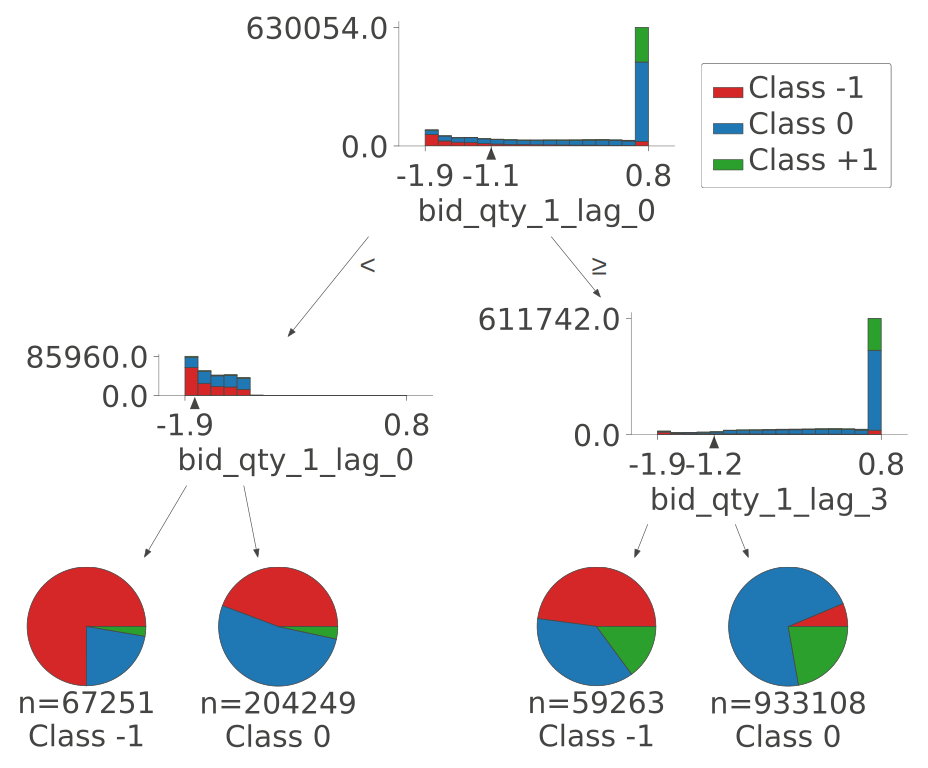
\includegraphics[width=0.7\textwidth]{./images/xgb_viz.pdf}
    \caption{A visualization of a single decision tree weak learner with max depth set to 2.}
    \label{fig:weaklearner}
\end{figure}

\subsection{Artificial Neural Networks}
Artificial Neural Networks are a broad class of machine learning model that can efficiently approximate
high dimensional non-linear functions. Perhaps the most famous example of an ANN (Artifical Neural Network)
is that of the Multi-Layer Perceptron, first introduced in \cite{ROSENBLATT1958}. The basic idea is to take some input
vector and successively project it onto new spaces with affine and then non-linear transformations.
An MLP with $N$ hidden layers can be defined mathematically as:
\begin{equation}
    \begin{aligned}
        f_i(x; W_i, b_i) &= \sigma_i(W_i x + b_i) \\
        f(x; W_1, W_2, ..., W_N, b_1, b_2, ..., b_N) &= f_N \circ f_{N-1} \circ ... \circ f_2 \circ f_1(x)
    \end{aligned}
\end{equation}
Where $W_i$  are learnable weight matrices, $b_i$ are learnable bias vectors, $\sigma_i$ are fixed non-linear activation functions and $\circ$ denotes function composition.
MLPs are powerful because, as \cite{HORNIK1989} shows, they are \textit{universal function approximators}.
This means that, with as few as one hidden layer and using arbitrary activation functions, 
they are capable of approximating any Borel measurable function from one finite dimensional space 
to another to any desired degree of accuracy, provided sufficiently many hidden units are available.
The weight matrices and bias vectors are learnt by minimizing some loss function.
If we denote our learnable parameters as $\theta$, then our loss function is given by:
\begin{equation}
   \mathcal{L} (\theta; x, y) := \frac{1}{n} \sum_{i=1}^{n} \ell(f(x_i; \theta), y_i)
\end{equation}
Where $\ell$ is some observation-wise loss that measures how well our model predicts
$y_i$ given corresponding input $x_i$.
For simple problems $\mathcal{L}$ is commonly a convex function and so gradient descent methods can be
used to perform the minimization. For example, for vanilla gradient descent, one might define the update rule as:
\begin{equation}
    \theta^{(t+1)} \gets \theta^{(t)} - \eta \nabla_\theta \mathcal{L}(\theta^{(t)})
\end{equation}
In practice the optimization problem is often not convex, with many local minima, and so alternative optimization methods
are often used, such as \textit{Stochastic Gradient Descent}, \cite{ROBBINS1951}, or \textit{ADAM}, \cite{ADAM2017}.
Stochastic Gradient Descent is a stochastic approximation of the gradient descent method, that
evaluates the gradient on a randomly sampled subset of the training data, instead of the entire training data.
It can be shown, \cite{ROBBINS1951}, that the stochastic approximation of the gradient converges in expectation to
the gradient evaluated on the entire training dataset.
This sub-sampling allows for fewer gradient evaluations and therefore faster training. Also the stochastic
nature of the algorithm means it is less likely to get stuck in local minima.
ADAM, first introduced in \cite{ADAM2017}, is a more advanced type of Stochastic Gradient Descent
that uses the concept of \textit{Momentum}, \cite{RUMELHART1986}. Momentum accumulates
the gradient from past updates to help guide the direction of the current step. It helps
to reduce oscillations during descent and often leads to faster convergence.

The ADAM update step is given by:
\begin{equation}
    \begin{aligned}
        m_{\theta}^{(t+1)} &\leftarrow \beta _{1}m_{\theta}^{(t)}+\left(1-\beta _{1}\right)\nabla_{\theta} \mathcal{L}(\theta^{(t)}) \\
        v_{\theta}^{(t+1)} &\leftarrow \beta _{2}v_{\theta}^{(t)}+\left(1-\beta _{2}\right)\left(\nabla_{\theta} \mathcal{L}(\theta^{(t)})\right)^{2} \\
        {\hat {m}}_{\theta} &={\frac {m_{\theta}^{(t+1)}}{1-\beta _{1}^{t}}} \\
        {\hat {v}}_{\theta} &={\frac {v_{\theta}^{(t+1)}}{1-\beta _{2}^{t}}} \\
        \theta^{(t+1)} &\leftarrow \theta^{(t)}-\eta {\frac {{\hat {m}}_{\theta}}{{\sqrt {{\hat {v}}_{\theta}}}+\delta }}.
    \end{aligned}
\end{equation}
So we see that ADAM uses exponential moving averages with decay factors $\beta_1$ and $\beta_2$ to accumulate first and
second gradient moments. Note that $\delta$ is some small constant, used to prevent zero division errors.

Using traditional differentiation methods, the $\nabla_\theta \mathcal{L}(\theta^{(t)})$ calculation would be very computationally
expensive and training would be too slow to be practical. Instead, an algorithm called \textit{backpropagation}, \cite{RUMELHART1986},
can be used to efficiently differentiate the network with respect to the weights and biases. 
Backpropagation is an efficient implementation of the chain rule for differentiation that uses
dynamic programming to avoid repeated calculations. The idea is to construct a \textit{computational graph},
which is a graph datastructure, where nodes represent functions and the edges represent function compositions.
So by doing a \textit{forward pass} of the graph, we are essentially evaluating the network given some input.
We then get an output, and do a \textit{backward pass} to accumulate gradients in an efficient way using the chain rule.
Backpropagation has computational complexity of the order of the number of edges in the computational graph,
so for large networks it scales very well and can be made to run extremely efficiently.

\subsection{Convolutional Neural Networks}

Convolutional Neural Networks (CNNs) are a specialized class of artificial neural 
networks designed primarily for processing structured grid data, such as images.
First introduced in \cite{LECUN1998}, CNNs have become a cornerstone in the field of
computer vision due to their ability to efficiently capture spatial hierarchies in data.

The fundamental building block of a CNN is the convolutional layer, which applies a
series of learnable filters (or kernels) to the input data.
Each filter \textit{convolves} across the input.
Mathematically, the output of a convolutional layer can be expressed as:
\begin{equation}
    h_{ij} = \sigma\left((W * x)_{ij} + b\right)
\end{equation}
where $W$ are the learnable filters, $b$ are the learnable biases,
$*$ denotes the convolution operation, and $\sigma$ is a non-linear 
activation function applied element-wise.
Note that for a $k\times k$ filter, the discrete convolution operation is defined as:
\begin{equation}
    (W * x)_{ij} := \sum_{m=-k}^{k}\sum_{n=-k}^{k} W_{mn} x_{i-m, j-n}
\end{equation}
So essentially we're sliding a window/filter over our 2D data and taking the dot product
at each position, resulting in a new 2D output for each filter.
This means the number of 2D outputs (\textit{channels}) is equal to the number of filters
for that layer.
The convolutional operation is a vector product and is differentiable with respect to
the filters, so we can simply apply gradient descent, just the same as with ANNs,
to learn our filters and biases.

In addition to convolutional layers, we also introduce \textit{pooling layers} 
which down-sample the spatial dimensions of the input, reducing computational
complexity and aiding in hierarchical feature extraction. 
The most common type of pooling is max-pooling, defined as:
\begin{equation}
    h_{ij} = \max_{(m,n) \in P_{ij}} x_{mn}
\end{equation}
where \(P_{ij}\) represents a pooling region around position $(i,j)$.

CNNs are powerful because they leverage three important ideas: local receptive fields, 
shared weights, and spatial subsampling. These ideas enable CNNs to only look at relevant information,
be much more computationally efficient and also to be invariant to small translations, scale, and distortions, \cite{ABRAMS2017}.

\subsection{Long Short-Term Memory}

First introduced in \cite{HOCHREITER1997}, a Long Short-Term Memory 
is a special type of Recurrent Neural Network.
RNNs are neural networks that take in sequences of input iteratively. At each iteration,
they take in the previous \textit{hidden state} and the current input and then update
the hidden state and give an output. This hidden state mechanism allows them 
to \textit{remember} long-term dependencies between inputs and they are often used to learn temporal dependencies in timeseries data.
One of the most famous simple RNNs is the Jordan network, introduced in \cite{JORDAN1997},
where the hidden state at each iteration, $h_t$ and the output $y_t$ are given by:
\begin{equation}
    \begin{aligned}
        h_t &= \sigma_h(W_h x_t + U_h y_{t-1} + b_h)  \\
        y_t &= \sigma_y(W_y h_t + b_y)
    \end{aligned}
\end{equation}
where $x_t, h_t, y_t$ are the input, hidden state and output at iteration $t$ respectively.
$W, U$ and $b$ are all learnable parameter matrices/vectors and $\sigma_h$ and $\sigma_y$ are activation functions.
Whilst in theory, simple RNNs should be able to remember any length dependency, in practice
they suffer from the \textit{vanishing gradients problem}, \cite{PASCANU2013}, where
gradients converge to zero during training, and therefore learning stops.
LSTMs were designed to address this problem, with special \textit{forget gates} which
learn to forget irrelevant information.
The most common type of LSTMs are composed of an \textit{input gate}, \textit{output gate}, \textit{forget gate}
and a \textit{cell}. The cell learns the information and the other gates regulate the flow of information from/to the cell.
Mathematically this looks like:
\begin{equation}
    \begin{aligned}
        f_t &= \sigma_g(W_f x_t + U_f h_{t-1} + b_f) \\
        i_t &= \sigma_g(W_i x_t + U_i h_{t-1} + b_i) \\
        o_t &= \sigma_g(W_o x_t + U_o h_{t-1} + b_o) \\
        \tilde{c}_t &= \sigma_c(W_c x_t + U_c h_{t-1} + b_c) \\
                c_t &= f_t \odot c_{t-1} + i_t \odot \tilde{c}_t \\
        h_t &= o_t \odot \sigma_h(c_t)
    \end{aligned}
\end{equation}
where $\odot$ denotes the element-wise product, \cite{SCHMIDHUBER1999}.
So essentially we are just expanding on the idea of the RNN with more hidden state
for greater control over what information is learnt.
Just like any other neural network, RNNs and LSTMs can be trained by gradient descent
with backpropagation.


\section{Model Architectures}
In this section we introduce the specialized models we will be using for our classification problem.

\subsection{Orderbook Features}
Before we introduce our models, we first must introduce our features.
We seek to define feature vectors $\bm{x}_t \in \mathbb{R}^d$ which capture the relevant orderbook 
information relating to future mid-price movement. We can then learn a model of the form:
\begin{equation}
    \hat{y}(t) = \hat{f}(\bm{x}(t))
\end{equation}
that seeks to minimize some loss function w.r.t the true labels $y(t)$, i.e.
\begin{equation}
   \hat{f} = \arg \min_{f} \mathcal{L}(\bm{y}, f(X))
\end{equation}

\subsubsection{Raw Orderbook Features}
\cite{ZHANG2019} use the raw orderbook data for their model input i.e. $\bm{x}(t)$ takes the form:
\begin{equation}
    \bm{x}(t) =: \bm{x}_t = [p_{t, \ell}^A, q_{t, \ell}^A, p_{t, \ell}^B, q_{t, \ell}^B]_{\ell=1}^{L} \in \mathbb{R}^{4L}
    \label{LOB_feature_vector}
\end{equation}
where $L$ represents the maximum orderbook level in the data. For our data we have 10 orderbook
levels, so $L=10$. It is important to note that this is a non-stationary series.
It also combines price and volume information, which have different units, which is not ideal for most models.
Henceforth, we shall refer to this feature vector as the LOB (Limit OrderBook) feature vector.


\subsubsection{Orderflow Features}
\cite{KOLM2023} extend the idea of OFI, defined in (\ref{eBeA}), beyond the first level.
Define \footnote{We interchangeably use the notation $p_t := p(t)$.} the contribution of
the $n^\text{th}$ event at level $\ell$ on the (A)sk/(B)id side as: 
\begin{align}
    e_{t,\ell}^{A} &:=  I_{\{ p_{n, \ell}^A \leq p_{n-1,\ell}^A \}} q_{n}^A - I_{\{ p_{n, \ell}^A \geq p_{n-1, \ell}^A \}} q_{n-1, \ell}^A \\
    e_{t, \ell}^{B} &:= I_{\{ p_{n, \ell}^B \geq p_{n-1, \ell}^B \}} q_{n, \ell}^B - I_{\{ p_{n, \ell}^B \leq p_{n-1, \ell}^B \}} q_{n-1, \ell}^B
\end{align}
Then we define the Orderflow feature vector as:
\begin{equation}
    \bm{x}_t := [e_{t, \ell}^{A}, e_{t, \ell}^{B}]_{\ell=1}^L \in \mathbb{R}^{2L} \label{OF_feature_vector}
\end{equation}
This feature vector is stationary and is given in units of volume, so is consistent across dimensions.
It is also half the dimension of the LOB feature vector, a desirable property for the convergence of many models.
Henceforth, we shall refer to this feature vector as the OF (OrderFlow) feature vector.


\subsection{lrLOB \& lrOF}
For our use case, we will define two logistic regression models, one using the LOB feature vectors first introduced in \ref{LOB_feature_vector}
and the other using the OF features introduced in \ref{OF_feature_vector}. 
Henceforth we will refer to these models as lrLOB and lrOF respectively.
Of course, when dealing with timeseries modelling, it is also important to incorporate autoregressive
features that allow the model to see previous observations for some lookback window.
We define our lookback window to be the previous $T$ observations. We incorporate these into
our model by concatenating lagged versions of the feature vector, i.e. our model inputs will be:
\begin{equation}
    \bm{x}^{AR}_t = [\bm{x}_t; \bm{x}_{t-1}; \bm{x}_{t-2}; \cdots; \bm{x}_{T-1}] \in  \mathbb{R}^{dT}\label{AR_features}
\end{equation}
This will be the input to our logistic regression models.
The output will be $\hat{y}_t \in \{-1, 0, 1\}$.
Note that we choose $T=10$, since larger values of $T$ will hurt the convergence
of the fitting algorithm and take too much memory and too long to fit.
This is a major limitation of this model and in later sections we introduce models
designed to handle much larger lookback windows.
\clearpage

\subsection{xgbLOB \& xgbOF}
XGBoost, first introduced in \cite{XGBOOST2016}, is an extremely efficient implementation of Boosted Decision Trees.
We choose XGBoost as one of our models for several reasons.
Firstly XGBoost has been shown to be highly effective in a wide range of applications.
It has great representational capacity, with the ability to capture high dimensional, non-linear relationships
in the data, with tight control of overfitting.
It handles high dimensional data well, with feature sub-sampling helping to reduce overfitting.
It also has great explainability, with the ability to rank features by importance (which we will explore in a later section).
As an added bonus, it can be run on a GPU, allowing for very fast training and inference.
Interestingly there is little to no mention of its use for limit orderbook prediction in the literature,
and we believe it has great potential for this purpose.
XGBoost has many hyperparameters that one can tune. We fine-tune our models on validation data and 
present our fine-tuned hyperparameters along with their definitions here:
 \begin{itemize}
    \item \textbf{max depth} = 10. The max depth of each weak learner tree.
    \item \textbf{eta} = 0.1. Step size shrinkage used in update to prevent overfitting. After each boosting step, we can directly get the weights of new features, and eta shrinks the feature weights to make the boosting process more conservative.
    \item \textbf{data subsample ratio} = 0.8. The proportion of the training data that each weak learner can use.
    \item \textbf{column subsample ratio} = 0.8. The proportion of the features available when performing splits.
    \item \textbf{evaluation metric} = Multiclass classification error rate. The metric used during the boosting algorithm to determine weights.
\end{itemize}


Similar to our logistic regression models, we define two XGBoost models, one using the LOB feature vectors first introduced in \ref{LOB_feature_vector}
and the other using the OF features introduced in \ref{OF_feature_vector}. 
Henceforth we will refer to these models as xgbLOB and xgbOF respectively.
As before, we use the autoregressive feature concatenation introduced in \ref{AR_features}.
Through experimentation on the validation set, we find that setting $T := k$ gives best performance.
However, as with the logistic regression models, we are limited by memory. 
This time we are limited by GPU memory. Specifically we find that $T := 20$ is the maximum
feasible lookback for our setup and therefore we set  $T := \min(k, 20)$.
\clearpage

\subsection{DeepLOB}
First introduced in \cite{ZHANG2019}, the DeepLOB model is a deep neural network
that uses a combination of convolutional and LSTM layers to extract short and long term
features from the raw orderbook data.
In this section we give a general overview of this model, but we refer the interested
reader to \cite{ZHANG2019} for a more in-depth exposition.

Firstly, it is important to understand the structure of the model input in order
to understand the convolutional filter dimension choices.
The model input is a vertical concatenation of our LOB feature
vectors, denoted by $X_t \in \mathbb{R}^{T \times 4L}$, where $X_t :=$
\begin{equation*}
\begingroup
\setlength\arraycolsep{1pt}
\begin{bmatrix}
p_{t-T, 1}^A & q_{t-T, 1}^A & p_{t-T, 1}^B &  q_{t-T, 1}^B &  \cdots & p_{t-T, L}^A &  q_{t-T, L}^A & p_{t-T, L}^B & q_{t-T, L}^B\\
p_{t-(T-1), 1}^A & q_{t-(T-1), 1}^A & p_{t-(T-1), 1}^B &  q_{t-(T-1), 1}^B &  \cdots & p_{t-(T-1), L}^A &  q_{t-(T-1), L}^A & p_{t-(T-1), L}^B & q_{t-(T-1), L}^B\\
\vdots & \vdots & \vdots & \vdots & \ddots & \vdots & \vdots& \vdots & \vdots\\
p_{t-1, 1}^A & q_{t-1, 1}^A & p_{t-1, 1}^B &  q_{t-1, 1}^B &  \cdots & p_{t-1, L}^A &  q_{t-1, L}^A & p_{t-1, L}^B & q_{t-1, L}^B\\
p_{t, 1}^A & q_{t, 1}^A & p_{t, 1}^B &  q_{t, 1}^B &  \cdots & p_{t, L}^A &  q_{t, L}^A & p_{t, L}^B & q_{t, L}^B\\
\end{bmatrix}
\endgroup
\end{equation*}
Note that if we reshape and flatten this matrix, we recover our autoregressive LOB feature vector defined in (\ref{AR_features}),
however in this case, we can use a much larger lookback without running out of memory, so we set $T=100$.

The DeepLOB model is comprised of three main modules, a convolutional module, an inception module and
an LSTM module. The output is then fed into a final linear layer before being passed through a softmax
function to give probabilities of each class, where the function $\text{softmax}: \mathbb{R}^d \to \Delta^{d-1}$
is defined element-wise as:
\begin{equation}
   \text{softmax}(x)_i = \frac{\exp(x_i)}{\sum_{j=1}^{d} \exp(x_j)}
\end{equation}

$\text{LeakyReLU}(x) := \max(0, x) + 0.01 * \min(0, x)$, \cite{MAAS2013}, activation functions are used between each layer to introduce non-linearity.
Batch normalization is also used to ensure stable training.
We use the ADAM optimizer, \cite{ADAM2017}, with learning rate set to $0.0001$ and the Cross Entropy Loss, \cite{CROSSENTROPYLOSS},
which is essentially a weighted log-softmax.

We present a schematic of the DeepLOB model in Figure \ref{fig:DeepLOB} and give a more in-depth explanation
of the three main modules below.
\clearpage

\subsubsection{DeepLOB Main Modules}
\begin{multicols}{2}
\textbf{Convolutional Module:}
 \begin{itemize}
    \item Conv 1 aggregates price and volume information for each level for each side;
    \item Conv 2 aggregates information across side for each level;
    \item Conv 3 aggregates information across the whole orderbook.
\end{itemize}
The convolutional blocks use horizontal filters of dimension $1 \times 2$ with stride $1 \times 2$, in order
to combine price and volume information. Then they use vertical $4 \times 1$ convolutional filters to combine
information across time, $4$ timesteps at a time. Then the final convolutional block uses a $1 \times 10$ convolutional
filter to combine information across all 10 levels of the orderbook.

\textbf{Inception Module:}
The inception module has three blocks. The $1 \times 1$ filters increase the dimensionality of
the input and then the $3 \times 1$ and $5 \times 1$ simulate moving averages.
The main idea is to simulate a \textit{Network-In-Network}, \cite{MIN2014}.
A Network-In-Network essentially replaces the convolution operation with a small MLP
that is shared among all convolutional windows. The output is obtained by sliding the MLP
over the input in a similar manner as CNN.
The outputs of each inception block are then concatenated and reshaped into a $\mathbb{R}^{T \times 192}$ timeseries
which is then fed into the LSTM module.

\textbf{LSTM Module:}
The LSTM module is comprised of an LSTM layer with 64 hidden units. The purpose
of this layer is to capture long term dependencies from the inception output.

\columnbreak
\begin{figure}[H]
    \centering
    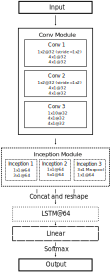
\includegraphics[width=0.50\textwidth]{./images/deepLOB_architecture_long.pdf}
    \caption{DeepLOB model architecture overview. Note: 1x2@32 denotes a convolutional layer with 32 filters and kernel size 1x2.}
    \label{fig:DeepLOB}
\end{figure}
\end{multicols}
\clearpage

\subsection{DeepOF}
Introduced in \cite{KOLM2023}, DeepOF is a modification of the DeepLOB architecture, using
OF features, rather than LOB features. \cite{KOLM2023} show that using orderflow
instead of the raw orderbook representation leads to better performance.
The DeepOF input is given by:

\begin{equation}
X_{t} := \begin{bmatrix}
e_{t-T, 1}^A & e_{t-T, 1}^B &   \cdots & e_{t-T, L}^A & e_{t-T, L}^B \\
e_{t-(T-1), 1}^A & e_{t-(T-1), 1}^B &   \cdots & e_{t-(T-1), L}^A & e_{t-(T-1), L}^B \\
\vdots & \vdots & \ddots & \vdots & \vdots \\
e_{t-1, 1}^A & e_{t-1, 1}^B &  \cdots & e_{t-1, L}^A & e_{t-1, L}^B \\
e_{t, 1}^A & e_{t, 1}^B &  \cdots & e_{t, L}^A & e_{t, L}^B \\
\end{bmatrix} \in \mathbb{R}^{T \times 2L}
\label{DeepLOB_input}
\end{equation}
where we have extended the tick level orderflow definition from (\ref{eBeA}) to any arbitrary orderbook level, $\ell$:
\begin{equation}
    \begin{aligned}
        e_{t, \ell}^B &:= I_{\{p_{t, \ell}^B \ge p_{t-1, \ell}^B\}} q_{t, \ell}^B - I_{\{p_{t, \ell}^B \le p_{t-1, \ell}^B\}} q_{t-1, \ell}^B \\
        e_{t, \ell}^A &:= I_{\{p_{t, \ell}^A \le p_{t-1, \ell}^A\}} q_{t, \ell}^A - I_{\{p_{t, \ell}^A \ge p_{t-1, \ell}^A\}} q_{t-1, \ell}^A
    \end{aligned}
\end{equation}
In terms of model architecture, the DeepOF model is the same as the DeepLOB model, except without
the first convolutional block, Conv 1. Recall that this block aggregates the price and volume information
from the LOB input, so by using OF input, we have essentially aggregated the price and volume information manually
using a predefined feature transform that has been shown to be predictive of mid-price movement. \cite{CONT2013}, \cite{KOLM2023}.

\section{Methodology}

\subsection{Sliding Window Setup}
We use a sliding window evaluation method, with train, validation and testing splits.
See Figure \ref{fig:slidingwindow} for a visual representation
of the splits.

\begin{figure}[htpb]
    \centering
    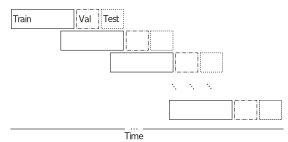
\includegraphics[width=1.0\textwidth]{./images/sliding_window.pdf}
    \caption{Sliding window visualization.}
    \label{fig:slidingwindow}
\end{figure}

So using this method we are able to validate and test on almost the entire dataset,
and only train on recent, relevant information. Note that we leave gaps between the train,
val and test blocks to avoid data leakage from features that look back in time.
We fix the length of the initial training window to 48 hours and the validation and testing windows to 24 hours each.

The general testing procedure will be to train on the training set, then fine-tune our hyperparameters using
the validation set, then once all of our hyperparameters have been chosen, 
we will test on the test set. Of course this means there will be a gap of 24 hours between our training
and testing data. We could alternatively merge the training and validation data once hyperparameter tuning is
complete and then re-train our models on the merged data before testing. However, leaving this gap
will provide an extra guarantee of robustness and provide a better picture of the out of sample
performance of our models.

\subsection{Data Normalization}
For several of our models, data normalization is important in order to ensure stable training
and convergence. \cite{LUCCHESE2024} and \cite{ZHANG2019} use five day rolling window normalization
whereas \cite{KOLM2023} use $z$-scores calculated using the training data.
We find the rolling window normalization method to give worse performance, since it transforms
our data in a non-linear way and so, for example, periods of no price change are
no longer flat. So following \cite{KOLM2023}, for each train-val-test window we calculate the 
sample mean and standard deviation of the training data, and use these to scale the training,
validation and testing data via $z$-scores.
% , i.e 
% \begin{equation}
%     \begin{aligned}
%         \hat{\mu}_{\text{train}} &:= \frac{1}{n_{\text{train}}} \sum_{i=1}^{n_{\text{train}}} X[i, :] \\
%         \hat{\sigma}_{\text{train}} &:= \frac{1}{n_{\text{train}}} \sum_{i=1}^{n_{\text{train}}} (X[i, :] - \hat{\mu}_{\text{train}})^2 \\
%         \tilde{X}_{\text{train}} &:= \frac{X_{\text{train}} - \hat{\mu}_{\text{train}}}{\hat{\sigma}_{\text{train}}} \\
%         \tilde{X}_{\text{val}} &:= \frac{X_{\text{val}} - \hat{\mu}_{\text{train}}}{\hat{\sigma}_{\text{train}}} \\
%         \tilde{X}_{\text{test}} &:= \frac{X_{\text{test}} - \hat{\mu}_{\text{train}}}{\hat{\sigma}_{\text{train}}}
%     \end{aligned}
% \end{equation}

\subsection{Choice of label discretization parameter}
Following \cite{LUCCHESE2024}, we set our discretization parameter, $\epsilon$, from (\ref{desc})
for each $k$ and train-val-test window, $w$, so that the classes are roughly balanced. i.e.
\begin{equation}
    \epsilon := \epsilon_{k, w} := \frac{|\hat{F}_{k, w}^{-1}(\frac{1}{3})| + \hat{F}_{k, w}^{-1}(\frac{2}{3})}{2}
\end{equation}
Where $\hat{F}_{k, w}$ is the empirical distribution of the training set $\ell(t)$, (\ref{smoothed_returns}), smoothed returns 
for prediction horizon $k$, and window $w$.


\subsection{Model Training}
Our DeepLOB and DeepOF models were trained with PyTorch, \cite{PYTORCH2017},
on an Nvidia RTX 3060 12GB with 64GB memory and a 14-core 20-thread Intel i5 13600K.
We use the ADAM optimizer, \cite{ADAM2017}, with learning rate set to $0.0001$.
For our loss function we use the Cross Entropy Loss, \cite{CROSSENTROPYLOSS}.
We trained our models until the validation loss plateaued and then used
the model from the epoch with highest validation loss.
% Our model 
% input is $(minibatch, C)$
% $$
% l_{n} = -w_{y_{n}} \log \frac{\exp(x_{n, y_{n}})}{\sum_{c=1}^C \exp(x_{n, c})softmax
% $$
% $$
% l(x, y) = \sum_{n=1}^N \frac{1}{\sum_{m=1}^N w_{y_{m}}} l_{n}
% $$
% ...
\clearpage

\section{Results}

\subsection{Classification Metrics}

Recall that this is a multi-class classification problem, with our three classes,
$-1$, for negative smoothed mid-price change, $0$ for insignificant smoothed mid-price change and $+1$ for positive mid-price change. 
This is an imbalanced problem, where we have up to $4 \times$ more $0$ labels for small $k$ compared with
$-1$ or $+1$ labels, since small time frames often mean no significant price change.
For this reason, accuracy is perhaps not the only metric we should care about.
In this case, \textit{precision}, \textit{recall} and \textit{F1} scores are often more insightful, \cite{HASTIE2001}.
Precision for class $ c $ is defined as:
\begin{equation}
\text{Precision}_c := \frac{\text{TP}_c}{\text{TP}_c + \text{FP}_c}
\end{equation}
where:
\begin{itemize}
    \item $ \text{TP}_c $ is the number of true positives for class $c$.
    \item $ \text{FP}_c $ is the number of false positives for class $c$.
\end{itemize}
So essentially, precision says: \textit{``out of all the times that we guessed class $c$, how many times were we correct?''}

Recall for class $c$ is defined as:
\begin{equation}
\text{Recall}_c := \frac{\text{TP}_c}{\text{TP}_c + \text{FN}_c}
\end{equation}
where:
\begin{itemize}
    \item $ \text{TP}_c $ is the number of true positives for class $c$.
    \item $ \text{FN}_c $ is the number of false negatives for class $c$.
\end{itemize}
So essentially, recall says: \textit{``out of all the times the true class was $c$, how many times did we predict it correctly?''}

F1-score for class $ c $ is the harmonic mean of precision and recall, defined as:
\begin{equation}
\text{F1-score}_c := 2 \cdot \frac{\text{Precision}_c \cdot \text{Recall}_c}{\text{Precision}_c + \text{Recall}_c}
\end{equation}

To get the overall performance across all classes, we can compute the macro-averaged precision, recall, and F1-score:
\begin{equation}
\text{Macro-Precision} := \frac{1}{3} \sum_{c \in \{-1,0,+1\}} \text{Precision}_c
\end{equation}

\begin{equation}
\text{Macro-Recall} := \frac{1}{3} \sum_{c \in \{-1,0,+1\}} \text{Recall}_c
\end{equation}

\begin{equation}
\text{Macro-F1-score} := \frac{1}{3} \sum_{c \in \{-1,0,+1\}} \text{F1-score}_c
\end{equation}

i.e. the unweighted mean. We can also define the weighted-average which weights each classes'
score according to their support. (Support for class $c$ is the number of instances of that class in the ground truth test labels).

\subsection{Model Results}
As previously stated, we train our models on the training windows, then validate
and tune our hyperparameters on the validation windows and then test on the test windows.
We present the results of the models on the test windows here.

We calculate the macro-averaged metrics on the test set for $k \in \{4, 10, 50, 200\}$ and present
the results in tables \ref{macro_table_1} - \ref{macro_table_4}. For brevity, we only present the results for BTCUSDT here. We will delve deeper
into the comparative performance of each model for different trading pairs later on. See appendix for un-averaged model results for all trading pairs.


\begin{table}[H]
\resizebox{0.99\textwidth}{!}{
\begin{tabular}{llllll}
\toprule
accuracy & precision & recall & f1-score & support & model \\
\midrule
\textbf{0.87}(0.03) & \textbf{0.91}(0.03) & \textbf{0.74}(0.01) & \textbf{0.80}(0.01) & 647295(30003) & \textbf{xgbOF} \\
0.79(0.04) & 0.75(0.05) & 0.68(0.02) & 0.70(0.01) & 647295(30003) & xgbLOB \\
0.84(0.04) & 0.87(0.02) & 0.70(0.01) & 0.76(0.01) & 647289(30003) & lrOF \\
0.69(0.07) & 0.66(0.08) & 0.60(0.07) & 0.59(0.06) & 647289(30003) & lrLOB \\
0.86(0.03) & 0.88(0.03) & \textbf{0.74}(0.01) & 0.79(0.0) & 647199(30003) & deepOF \\
0.75(0.2) & 0.73(0.22) & 0.70(0.04) & 0.69(0.17) & 647199(30003) & deepLOB \\
\bottomrule
\end{tabular}
}
\caption{Mean macro averaged BTCUSDT test set classification results across windows for $\bm{k=4}$. (Standard deviations are given in parenthesis).}
\label{macro_table_1}
\end{table}

\begin{table}[H]
\resizebox{0.99\textwidth}{!}{
\begin{tabular}{llllll}
\toprule
accuracy & precision & recall & f1-score & support & model \\
\midrule
\textbf{0.80}(0.03) & \textbf{0.84}(0.04) & 0.75(0.01) & \textbf{0.78}(0.02) & 647289(30003) & \textbf{xgbOF} \\
0.72(0.02) & 0.71(0.02) & 0.71(0.01) & 0.71(0.01) & 647289(30003) & xgbLOB \\
0.76(0.04) & 0.81(0.03) & 0.72(0.01) & 0.74(0.02) & 647289(30003) & lrOF \\
0.58(0.07) & 0.62(0.05) & 0.62(0.04) & 0.57(0.08) & 647289(30003) & lrLOB \\
0.79(0.03) & 0.81(0.02) & \textbf{0.76}(0.01) & 0.77(0.01) & 647199(30003) & deepOF \\
0.74(0.06) & 0.76(0.04) & 0.71(0.05) & 0.72(0.06) & 647199(30003) & deepLOB \\
\bottomrule
\end{tabular}
}
\caption{Mean macro averaged BTCUSDT test set classification results across windows for $\bm{k=10}$.}
\label{macro_table_2}
\end{table}

\begin{table}[H]
\resizebox{0.99\textwidth}{!}{
    \begin{tabular}{llllll}
    \toprule
    accuracy & precision & recall & f1-score & support & model \\
    \midrule
    0.64(0.04) & \textbf{0.65}(0.03) & 0.62(0.01) & 0.63(0.02) & 647279(30003) & xgbOF \\
    0.56(0.04) & 0.57(0.03) & 0.58(0.04) & 0.53(0.06) & 647279(30003) & xgbLOB \\
    0.57(0.05) & 0.62(0.03) & 0.55(0.0) & 0.55(0.02) & 647289(30003) & lrOF \\
    0.51(0.06) & 0.52(0.03) & 0.54(0.03) & 0.46(0.06) & 647289(30003) & lrLOB \\
    \textbf{0.66}(0.03) & \textbf{0.65}(0.02) & \textbf{0.65}(0.02) & \textbf{0.65}(0.02) & 647199(30003) & \textbf{deepOF} \\
    0.57(0.07) & 0.58(0.04) & 0.57(0.07) & 0.55(0.09) & 647199(30003) & deepLOB \\
    \bottomrule
    \end{tabular}
}
\caption{Mean macro averaged BTCUSDT test set classification results across windows for $\bm{k=50}$.}
\label{macro_table_3}
\end{table}

\begin{table}[H]
\resizebox{0.99\textwidth}{!}{
    \begin{tabular}{llllll}
    \toprule
    accuracy & precision & recall & f1-score & support & model \\
    \midrule
    0.52(0.04) & 0.53(0.03) & 0.50(0.01) & 0.51(0.01) & 647279(30003) & xgbOF \\
    0.46(0.04) & 0.45(0.02) & 0.48(0.02) & 0.40(0.04) & 647279(30003) & xgbLOB \\
    0.48(0.05) & 0.50(0.02) & 0.46(0.01) & 0.45(0.01) & 647289(30003) & lrOF \\
    0.44(0.05) & 0.45(0.04) & 0.47(0.03) & 0.39(0.04) & 647289(30003) & lrLOB \\
    \textbf{0.56}(0.03) & \textbf{0.56}(0.02) & \textbf{0.55}(0.02) & \textbf{0.55}(0.02) & 647199(30003) & \textbf{deepOF} \\
    0.49(0.05) & 0.48(0.04) & 0.49(0.06) & 0.47(0.05) & 647199(30003) & deepLOB \\
    \bottomrule
    \end{tabular}
}
\caption{Mean macro averaged BTCUSDT test set classification results across windows for $\bm{k=200}$.}
\label{macro_table_4}
\end{table}

Overall we observe very decent performance with clear predictability. We see that for $k=4$ and $k=10$ 
xgbOF is the clear winner. We then see that deepOF takes over for $k=50$ and  $k=200$.
To give a clearer picture of comparative performance across windows, we plot the macro averaged
precision, recall and F1 for each trading pair, for each window and for each $k$ in Figures \ref{macro_plots_1} - \ref{macro_plots_4}.


We see that for $k=4$ and $k=10$, generally, xgbOF has the best precision and deepLOB has the best recall, with very similar
F1 scores. We also observe that, in general the models perform similarly for different trading pairs, with model rankings generally preserved,
although we do see a slightly decreased performance for trading pairs with lower trade volume. It seems that the general performance of our models
is an increasing function of trading pair liquidity when measured using macro F1.
This is an interesting result, and suggests that perhaps higher volume trading pairs are more predictable.

As we increase $k$ to $50$ and then $200$, we see that the deepOF model starts pulling away from the other models for all metrics.
This is perhaps due to the fact that deepOF has a much larger, $T=100$, lookback, whereas (due to memory constraints) our xgbOF model
has lookback $T = \min(k, 20) = 20$ for $k= 50, 100$.
We see that xgbOF and deepOF give the most stable results across windows in terms of variation. We see lrLOB has high variation
and performs poorly. Interestingly lrOF performs very well, often beating out the much larger deepLOB and xgbLOB models.
It is clear that the OF representation is far superior, since all OF based models generally exhibit superior performance
(when not constrained by lookback).

Of course, whilst macro-averaging gives a good overall idea of comparative performance, it averages performance across classes,
so therefore we don't yet have a clear picture of how our models perform comparatively for each class.
In Figures \ref{BTCUSDT_cm} - \ref{SOLUSDT_cm} we present confusion matrices, with counts summed across windows.

Again we see that for smaller $k$ values, this is a very imbalanced classification problem, with the majority
of the labels being class $0$, i.e. stationary mid-price change. We see that as we increase $k$ the distribution
of labels spreads out more equally across classes. We also observe that, all of our confusion matrices have most weight
along their diagonals, which is good news and means our models all perform better than randomly guessing.
We see that the distributions are symmetric for the $+1$ and $-1$ classes so henceforth, in our analysis
we will group these classes together and refer to them as the non-zero classes.

Recall that precision is defined as the number of correctly predicted labels for a class divided by the number of predicted labels for that
class, and recall is the number of correctly predicted labels for a class divided by the total number of labels for that class.
Using a poker analogy, precision tells us, out of all the times that we played a hand, what proportion of times did we win. Recall
tells us, out of all the times that we had a winning hand, how many times did we play and win.
So for a trading scenario, what we really care about is precision of the $+1$ and $-1$ classes, since for most applications, it would
be much more harmful to play and lose, rather than not play and miss a winning hand.
We see that the precision of the non-zero classes is much higher than the precision of the zero class, whereas the recall of the
non-zero classes is much lower than the recall of the zero class. This is due to the imbalanced nature of our labels, and we
see that, as we increase $k$, the precision and recall get closer. The precision of the non-zero classes is around 90\% for our best models for
small $k$, which is a great result for the reasons mentioned above.

We see that, as we move across trading pairs, we start seeing less weight on the zero labels and more predictions
for the non-zero classes. This is perhaps due to the fact that, for our test data, MATICUSDT and SOLUSDT have more balanced support, compared with BTCUSDT and ETHUSDT. i.e. the distribution of the true labels is less imbalanced for MATICUSDT and SOLUSDT.
This is perhaps due to MATICUSDT and SOLUSDT having higher volatility over our testing windows, so fewer non-zero price changes.

\begin{figure}[htpb!]
    \centering
    \includegraphics[width=0.93\textwidth]{./images/macro_results_k=4.pdf}
    \caption{Comparing the macro averaged precision, recall and F1 score on the unseen test set for each window, for each trading pair, for $k=4$.}
    \label{macro_plots_1}
\end{figure}

\begin{figure}[htpb!]
    \centering
    \includegraphics[width=1.0\textwidth]{./images/macro_results_k=10.pdf}
    \caption{Comparing the macro averaged precision, recall and F1 score on the unseen test set for each window, for each trading pair, for $k=10$.}
    \label{macro_plots_2}
\end{figure}

\begin{figure}[htpb!]
    \centering
    \includegraphics[width=1.0\textwidth]{./images/macro_results_k=50.pdf}
    \caption{Comparing the macro averaged precision, recall and F1 score on the unseen test set for each window, for each trading pair, for $k=50$.}
    \label{macro_plots_3}
\end{figure}

\begin{figure}[htpb!]
    \centering
    \includegraphics[width=1.0\textwidth]{./images/macro_results_k=200.pdf}
    \caption{Comparing the macro averaged precision, recall and F1 score on the unseen test set for each window, for each trading pair, for $k=200$.}
    \label{macro_plots_4}
\end{figure}

\begin{figure}[htpb!]
    \centering
    \includegraphics[width=1.0\textwidth]{./images/BTCUSDT_confusion_matrices.pdf}
    \caption{BTCUSDT confusion matrices. Note that counts are summed across windows.}
    \label{BTCUSDT_cm}
\end{figure}

\begin{figure}[htpb!]
    \centering
    \includegraphics[width=1.0\textwidth]{./images/ETHUSDT_confusion_matrices.pdf}
    \caption{ETHUSDT confusion matrices. Note that counts are summed across windows.}
    \label{ETHUSDT_cm}
\end{figure}

\begin{figure}[htpb!]
    \centering
    \includegraphics[width=1.0\textwidth]{./images/MATICUSDT_confusion_matrices.pdf}
    \caption{MATICUSDT confusion matrices. Note that counts are summed across windows.}
    \label{MATICUSDT_cm}
\end{figure}

\begin{figure}[htpb!]
    \centering
    \includegraphics[width=1.0\textwidth]{./images/SOLUSDT_confusion_matrices.pdf}
    \caption{SOLUSDT confusion matrices. Note that counts are summed across windows.}
    \label{SOLUSDT_cm}
\end{figure}


\subsection{Feature Importances}
Another advantage of using a decision-tree-based model is that we get easily explainable
feature importances. During training, we split the tree at each level, using the feature
that gives us the best partition according to some metric. We can use this fact
to rank features based on the number of times a feature was used to split the tree. We
denote this count as the \textit{weight} of the feature.
More influential features will have a higher weight since they are the best discriminators
of the data.

We plot the top 10 LOB features for xgbLOB BTCUSDT in Figure \ref{top_10_lob_features} for different $k$, prediction horizons.
We see that for the LOB features, across all $k$, the highest weight features are 
the bid and ask quantities at the first level. This is very interesting,
and tells us that for the LOB model the top levels of the orderbook are the most relevant.
As we increase $k$, we start seeing larger lags being more important.  Recall that due to memory constraints
we set $T=\min(k, 20)$, so the maximum lag is 19. For $k > 20$ it seems
we would certainly benefit from a larger lookback.
Also a very important note; the majority of the top 10 features are quantity features. Recall
that the LOB features are both quantity and price. Clearly this shows that the model
is not using the price features effectively, and this demonstrates the need for a better
representation, such as orderflow.

We also plot the top 10 OF features for xgbOF BTCUSDT in Figure \ref{top_10_of_features}.
Again we see that the first level features are the most influential. This is good to see,
since it confirms the commonly shared idea that the top of the orderbook has the
most impact on price movement. Again we also see that, as we increase $k$, larger lag features
start to appear.

Next we examine the distribution of weights over all non-zero weighted features in Figures \ref{all_lob_features}
and \ref{all_of_features}. Instead of ordering the features by weight, we now order the features
by their index. Recall the LOB features are:
\begin{equation*}
    [\text{ask}\_\text{price}\_\ell\_\text{lag}\_p, \text{ask}\_\text{qty}\_\ell\_\text{lag}\_p, \text{bid}\_\text{price}\_\ell\_\text{lag}\_p, \text{bid}\_\text{qty}\_\ell\_\text{lag}\_p]_{\ell = 1, ..., 10, p = 0, ..., T}
\end{equation*}
And the OF features are:
\begin{equation*}
    [\text{ask}\_\text{orderflow}\_\ell\_\text{lag}\_p, \text{bid}\_\text{orderflow}\_\ell\_\text{lag}\_p]_{\ell = 1, ..., 10, p = 0, ..., T}
\end{equation*}
Where $\ell$ indexes the orderbook level, and $p$ indexes the lag.
Note that in Figures \ref{all_lob_features} and \ref{all_of_features} we distinguish different feature groups using different colors.
Each color represent a unique (feature type, lag) pair, where feature type is either quantity or price for LOB and orderflow for OF.
So for example, the first color represents all price features with lag 0. This allows us to compare feature weights
for price vs. quantity features and also for different lags. Also since features are ordered by index, we can compare
feature weights across levels, e.g. the first bar in a color group represents the first level for that feature type and lag.

Firstly we note that in \ref{all_lob_features} only every other bar has significant weight. These bars are quantity features and
the price features have very small, often zero, weight for most levels and lags.
This shows that the model is hardly using the price features, further confirming
the inefficiency of the LOB representation. For both the OF representation and LOB representation we see that for each color the feature weights
are decreasing as we increase the feature index. This shows that the features at the top levels have highest weight, and evidences
the idea that deeper levels are less relevant for mid-price prediction.
We also see that the first few levels all have similar weight across colors. This shows that the first few levels of the orderbook
are roughly equally important across lags. For example, ask\_qty\_1\_lag\_9 has similar importance to ask\_qty\_1\_lag\_0. So we see
that using auto-regressive (lagged) features is important, but using deeper levels of the orderbook is less important.

Note that we do not distinguish between ask and bid features because we find them to be equally important.

\begin{figure}[htpb!]
    \centering
    \includegraphics[width=1.0\textwidth]{./images/xgboost_LOB_BTCUSDT_top_10_feature_importances.pdf}
    \caption{Top 10 XGBoost LOB Feature Importances for BTCUSDT, measured by weight = number of times a feature was split on.}
    \label{top_10_lob_features}
\end{figure}
\begin{figure}[htpb!]
    \centering
    \includegraphics[width=1.0\textwidth]{./images/xgboost_OF_BTCUSDT_top_10_feature_importances.pdf}
    \caption{Top 10 XGBoost OF Feature Importances for BTCUSDT, measured by weight = number of times a feature was split on.}
    \label{top_10_of_features}
\end{figure}


\begin{figure}[htpb!]
    \centering
    \includegraphics[width=0.9\textwidth]{./images/xgboost_LOB_BTCUSDT_all_feature_importances.pdf}
    \caption{All non-zero LOB feature importances for BTCUSDT, measured by weight = number of times a feature was split on.
    Note that the colors represent unique (feature type, lag) pairs, where feature type is either quantity or price and lag $\in \{0, ..., T\} $,
    e.g. the first color represents price features with lag 0.}
    \label{all_lob_features}
\end{figure}

\begin{figure}[htpb!]
    \centering
    \includegraphics[width=0.9\textwidth]{./images/xgboost_OF_BTCUSDT_all_feature_importances.pdf}
    \caption{All non-zero OF feature importances for BTCUSDT, measured by weight = number of times a feature was split on.
    Note that the colors represent unique lags, where lag $\in \{0, ..., T\} $. 
    E.g. the first color represents all features with lag 0.}
    \label{all_of_features}
\end{figure}

\subsection{Modelling Recommendations}
To conclude, we recommend the xgbOF model for shorter time horizons due its superior performance,
ease of use, interpretability, scalability and lower training time.
This is interesting since, to our knowledge, XGBoost is not mentioned in the literature for high frequency orderbook mid-price prediction.
It would be interesting to see how the xgbOF model compares with the models presented in \cite{ZHANG2019}, \cite{KOLM2023} and \cite{LUCCHESE2024} when trained on their data.


For longer time horizons deepOF was the clear winner. Whether this was due to superior ability to capture long term
temporal dependencies or the fact that our xgbOF had a cap on lookback due to memory constraints remains to be seen
and we recommend anyone looking to predict mid-prices at longer time horizons to try both models.

